\let\negmedspace\undefined
\let\negthickspace\undefined
\documentclass[journal]{IEEEtran}
\usepackage[a5paper, margin=10mm, onecolumn]{geometry}
%\usepackage{lmodern} % Ensure lmodern is loaded for pdflatex
\usepackage{tfrupee} % Include tfrupee package

\setlength{\headheight}{1cm} % Set the height of the header box
\setlength{\headsep}{0mm}     % Set the distance between the header box and the top of the text

\usepackage{gvv-book}
\usepackage{gvv}
\usepackage{cite}
\usepackage{amsmath,amssymb,amsfonts,amsthm}
\usepackage{algorithmic}
\usepackage{graphicx}
\usepackage{textcomp}
\usepackage{xcolor}
\usepackage{txfonts}
\usepackage{listings}
\usepackage{enumitem}
\usepackage{mathtools}
\usepackage{gensymb}
\usepackage{comment}
\usepackage[breaklinks=true]{hyperref}
\usepackage{tkz-euclide} 
\usepackage{listings}
% \usepackage{gvv}                                        
\def\inputGnumericTable{}                                 
\usepackage[latin1]{inputenc}                                
\usepackage{color}                                            
\usepackage{array}                                            
\usepackage{longtable}                                       
\usepackage{calc}                                             
\usepackage{multirow}                                         
\usepackage{hhline}                                           
\usepackage{ifthen}                                           
\usepackage{lscape}
\begin{document}

\bibliographystyle{IEEEtran}
\vspace{3cm}

\title{4.3.56}
\author{EE25BTECH11065 - Yoshita}
% \maketitle
% \newpage
% \bigskip
{\let\newpage\relax\maketitle}

\renewcommand{\thefigure}{\theenumi}
\renewcommand{\thetable}{\theenumi}
\setlength{\intextsep}{10pt} % Space between text and floats

\textbf{Question}:\\
Find the equation of the plane with intercepts 2, 3 and 4 on the x, y and z - axis respectively.\\
\bigskip

\textbf{Solution}:\\
The intercepts define three points on the plane, which we can label A, B, and C.
\begin{table}[H]    
  \centering
  \begin{tabular}{|c|c|}
\hline
\textbf{Name} & \textbf{Value} \\ \hline
$\vec{A}$ & $\myvec{2 & 1 \\0 & 3}$ \\ \hline
\end{tabular}

  \caption{Answers}
  \label{Answers}
\end{table}
The equation of the plane can also be written in the form
\[
\mathbf{n}^T \mathbf{x} = 1
\]
  where $\mathbf{n}$ is the normal vector.

Substituting the three intercept points $A = \myvec{2\\0\\0}$, 
$B = \myvec{0\\3\\0}$, and $C = \myvec{0\\0\\4}$ into this equation:

\begin{align}
\mathbf{n}^T \mathbf{A} &= 1 
\;\;\;\;\;\;\;\;\;\;\;\;\;\;\;\;\;
\implies \mathbf{n}^T \myvec{2\\0\\0} = 1 \\[6pt]
\mathbf{n}^T \mathbf{B} &= 1 
\;\;\;\;\;\;\;\;\;\;\;\;\;\;\;\;\;
\implies \mathbf{n}^T \myvec{0\\3\\0} = 1 \\[6pt]
\mathbf{n}^T \mathbf{C} &= 1 
\;\;\;\;\;\;\;\;\;\;\;\;\;\;\;\;\;
\implies \mathbf{n}^T \myvec{0\\0\\4} = 1
\end{align}

Combining these into a single matrix equation:
\[
\myvec{
    2 & 0 & 0 \\
    0 & 3 & 0 \\
    0 & 0 & 4
}
\mathbf{n}
=
\myvec{1\\1\\1}
\]

Solving, we obtain
\[
\mathbf{n} = 
\myvec{\tfrac{1}{2}\\[4pt]\tfrac{1}{3}\\[4pt]\tfrac{1}{4}}
\]

Hence, the plane equation 
\[
\mathbf{n}^T \mathbf{x} = 1 
\]
\[
\myvec{\tfrac{1}{2}\\[4pt]\tfrac{1}{3}\\[4pt]\tfrac{1}{4}}\mathbf{x} =1
\]

\begin{figure}[H]
\begin{center}
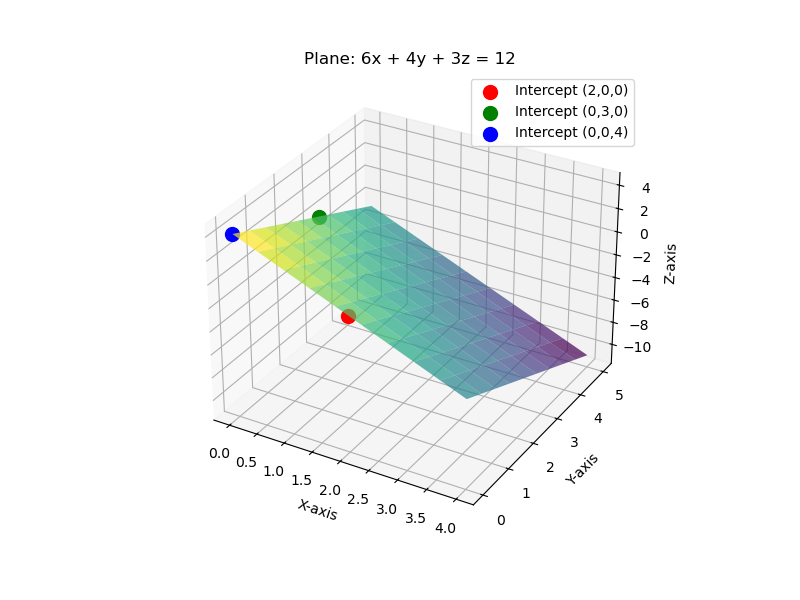
\includegraphics[width=0.7\columnwidth]{figs/fig2.png}
\end{center}
\caption{A plane intersecting the x, y, and z axes.}
\label{fig:Fig.1}
\end{figure}
\end{document}


